\documentclass[UTF8]{ctexart}%UTF8为中文使用的编码;%开头表示注释


%opening
\title{\heiti 这是标题}
\author{\kaishu 这是作者}
\date{\today}
\newtheorem{thm}{定理}%定义一个thm的环境
\usepackage{graphicx}
\usepackage{geometry}
\geometry{a4paper,centering,scale=0.8}%版心居中,长宽占页面的0.8倍。
\usepackage[format=hang,font=small,textfont=it]{caption}%改变图表标题格式,悬挂对齐方式(即编号向左突出)整体用小字号,而标题文本使用斜体(对汉字来说就是楷书)
\usepackage[nottoc]{tocbibind}%增加目录的项目:目录项本身、参考文献、索引等项目。nottoc取消了目录本身。
%以上为导言区,通常用来对文档的性质做一些设置,或自定义一些命令
\begin{document}
\maketitle
\tableofcontents%生成目录
\listoffigures%
\listoftables%产生图表的目录,!至少编译两遍
\begin{abstract}
这是摘要部分。
\end{abstract}

\section{第一节标题}
This is my first document.单个空行以示分行,多个空行以示分段,但是正文外的空行不表示任何意义。段前不用打空格,会自动完成文字的缩进,即使打了空格也会被忽略。

通常汉字后面的空格会被忽略,其他符号后面的空格则保留,左 右,left right.

欧几里得\footnote{欧几里得,约公元前330--275年。此为脚注部分}
\subsection{第一小节标题}
\begin{quote}
	\zihao{-5}\kaishu%改变字体
	quote环境,此为引用部分
\end{quote}

\begin{thm}[勾股定理]
	直角三角形斜边的平方等于两腰的平方和。需要现在导言区做定义。
\end{thm}
\noindent 禁止缩进

Happy \TeX ing.
\section{第二节标题:数学公式}
$a+b$%此类夹在行文中的公式称为“正文公式”或“行内公式”
%显示公式或列表公式
\begin{equation}
	a(b+c)=ab+ac
\end{equation}
$\angle ACB=\pi/2$
\begin{equation}
	AB^2=BC^2+AC^2.
	90^\circ
\end{equation}
\section{第三节标题:插入图片}

需在导言区引入graphicx宏包,就可以使用斜杠includegraphics命令插图了

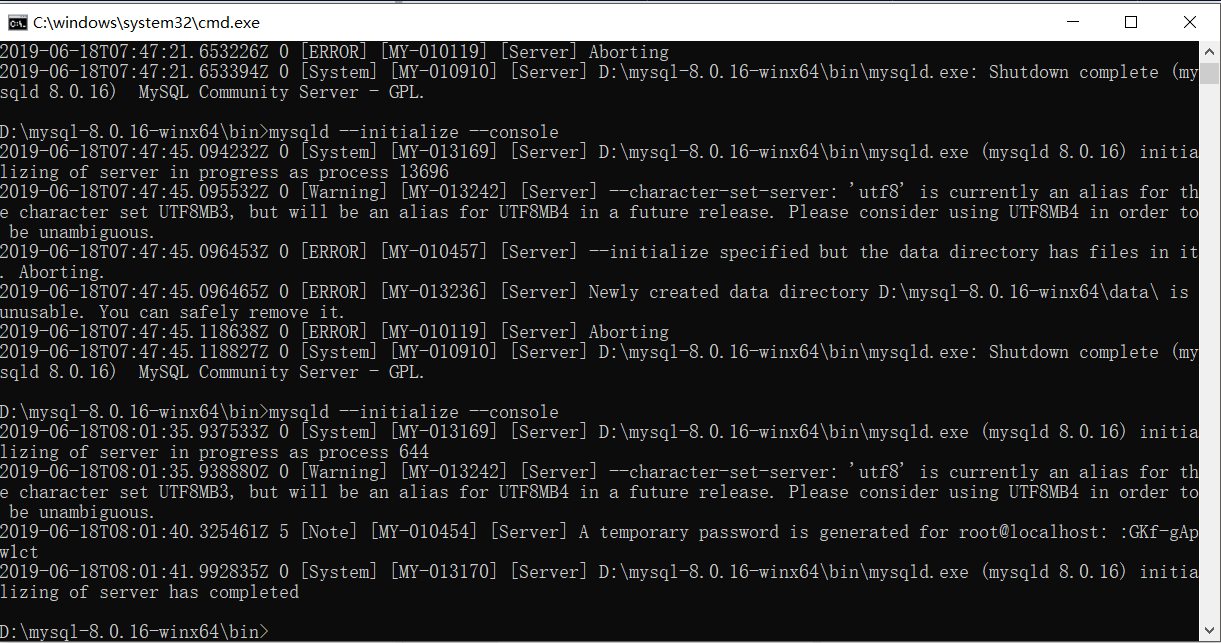
\includegraphics[width=6cm]{picture1.png}

参数包括scale=放缩因子、height=高度等,使用的图形文件格式与所使用的编译程序有关。图形放在根目录下才有效。
\begin{figure}[ht]%ht表示浮动体可以出现在环境周围的文本所在处(here)和一页的顶部(top)。
	\centering%表示后面的内容居中
	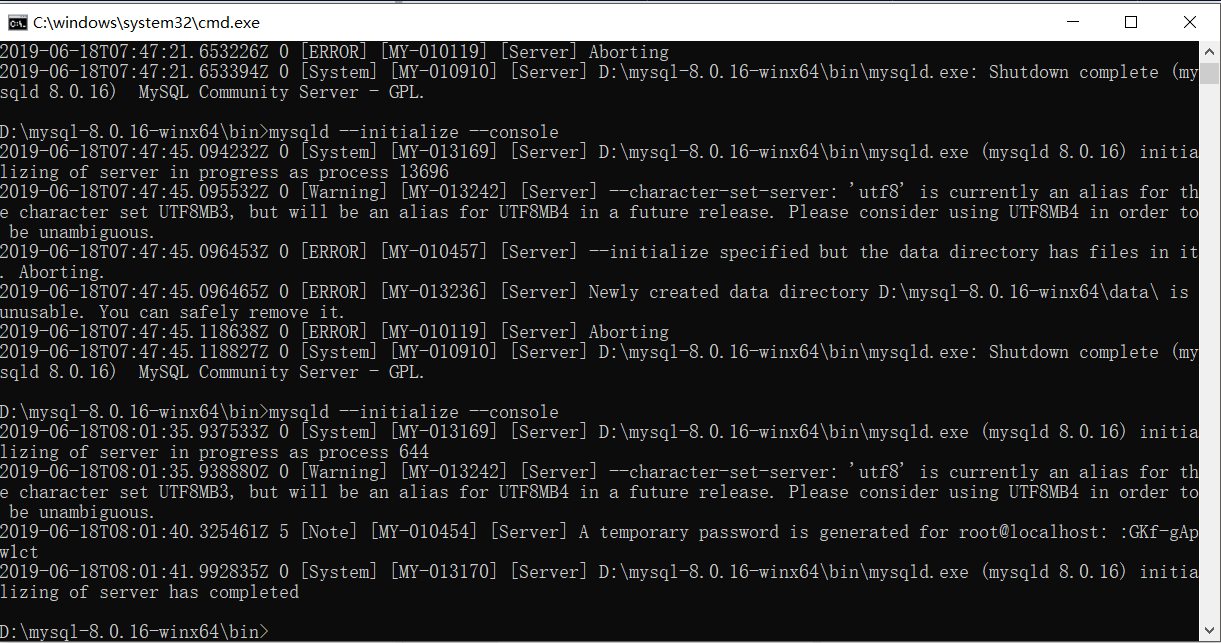
\includegraphics[scale=0.5]{picture1.png}
	\caption{宋赵爽在《周》注中做的炫图}%给插图加上自动编号和标题
	\label{fig:xiantu}%加标签,可在其他地方使用此图
\end{figure}
\section{第四节标题:插入表格}
插图可以用其他软件做好插入,但表格一般都还是直接在LaTeX里面完成的。制作表格,需要确定的是表格的行、列对齐模式和表格线,这是由tabular环境完成的。

\begin{tabular}{|rrr|}%表格有三列,都是右对齐。
	\hline%产生横线
	直角边 $a$ & 直角边 $b$ & 斜边 $c$\\
	\hline
	3& 4& 5\\
	5& 12& 13\\
	\hline
\end{tabular}
\section{第五节标题:文章格式}
设计页面尺寸可以使用geometry宏包
	
\end{document}
